\newpage
\section{CAPÍTULO III}
\section*{ANÁLISIS DE LA SITUACION ACTUAL}
%Introduccion del cap 3
En este capítulo, se realizará un análisis detallado de la situación actual de la empresa, centrándose en los problemas identificados en el capítulo anterior y su impacto en los procesos de atención al cliente. Utilizaremos diversas herramientas de análisis, como los diagramas de Proceso (DOP)  y de Actividades de Proceso (DAP), la espina de Ishikawa y el diagrama de Pareto, para comprender a fondo las causas subyacentes de los problemas y sus implicaciones en la eficiencia en la atención al cliente. Estos métodos permitirán identificar los puntos críticos del proceso y desarrollar una visión clara de las áreas que requieren mejoras para optimizar estos procesos específicos de la empresa, particularmente en las áreas de registro y facturación.

\subsection{3.1 Diagrama del proceso y diagrama de operación actual}
Para el análisis de la situación actual de le empresa, los diagramas de proceso (DOP) y Diagrama de Actividades de Procesos (DAP) son herramientas fundamentales para visualizar y comprender como se llevan a cabo los procesos dentro de la empresa.

\subsubsection*{3.1.1 Diagrama de operaciones de procesos (DOP)}
En el diagrama \ref{fig:DiagramaDOP} se proporciona una representación visual que describe el flujo de actividades en la atención al cliente, el registro de nuevos cliente y vehículos y la facturación. 
\begin{itemize}
    \item El tiempo total estimado (sin considerar el tiempo del servicio e inspección): 32 minutos
    \item Total estimado de tiempo (con el tiempo del servicio): 102 minutos
\end{itemize}


%El proceso comienza con la recepción del cliente, seguida del registro de entrada en la lista impresa, donde se recopilan los detalles del cliente y del vehículo. Luego, se lleva a cabo la evaluación del vehículo, que puede implicar la inspección visual y la identificación de problemas. Posteriormente, se crea una orden de trabajo que detalla los servicios solicitados por el cliente. 
%Una vez creada la orden de trabajo, se asigna el trabajo a un mecánico desocupado, quien se encarga de realizar el servicio solicitado. Tras la finalización del servicio, se realiza una inspección de calidad para asegurar que el trabajo se haya completado según los estándares establecidos.
%Una vez aprobada la inspección de calidad, el vehículo es despachado al cliente. Finalmente se hace la facturación o emisión de la boleta del servicio efectuado. Cada actividad en el proceso tiene un tiempo estimado de realización, lo que proporciona una indicación de la duración total del proceso y ayuda a identificar posibles áreas de mejora en términos de eficiencia y tiempos de espera.

%\begin{table}[H]
%    \captionsetup{labelformat=empty}
%    \caption[Diagrama de Proceos Actual (DOP)]{\textbf{Diagrama de Procesos Actual (DOP)}}
%    \begin{tabular}{p{7cm}c}
%        %\includesvg[width=1\textwidth]{imagenes/cap3/DOP1.svg} \\
%        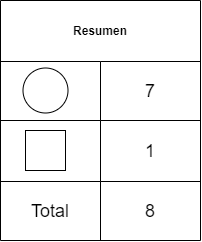
\includegraphics[width=6cm, height=8cm]{imagenes/cap3/DOPcap3Tabla.drawio.png} & 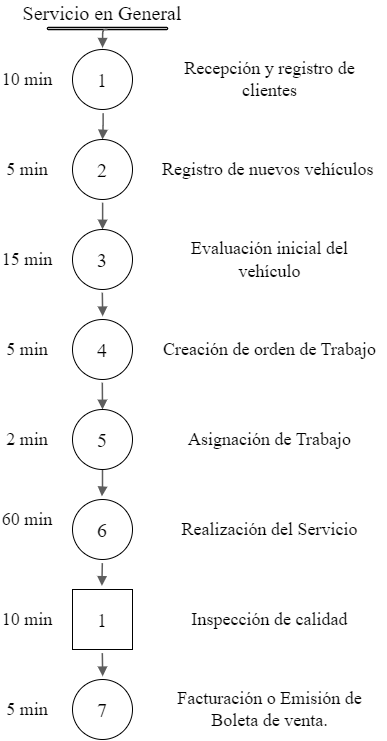
\includegraphics[width=8cm, height=18cm]{imagenes/cap3/DOPCap3.drawio.png} \\
%    \end{tabular}
%    \label{fig:diagramaDOP}
%\end{table}
\begin{figure}[H]
    \caption[Diagrama de Proceos Actual (DOP)]{Diagrama de Procesos Actual (DOP)}
    \centering
    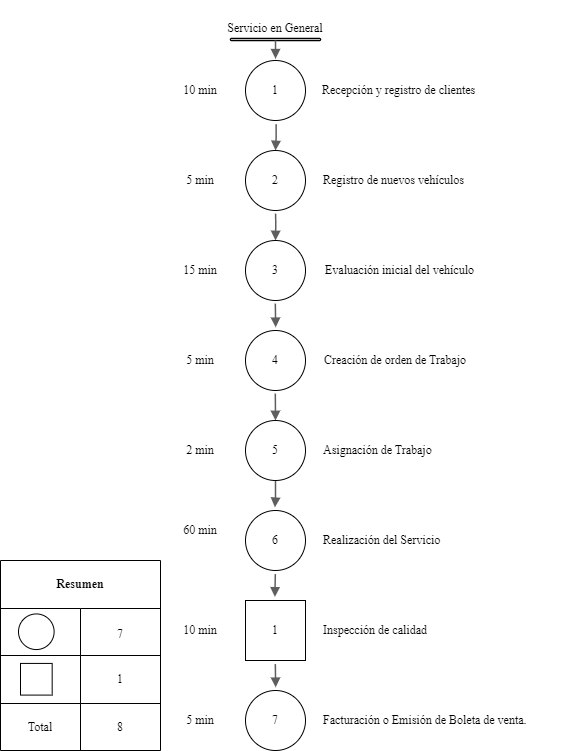
\includegraphics[width=12cm, height=15cm]{imagenes/cap3/DiagramaDOP.drawio.png}
    \label{fig:DiagramaDOP}
\end{figure}


%\begin{table}[H]
%\begin{tabular}{p{5cm}p{22cm}}
% &
% \captionsetup{labelformat=empty}
% \caption{Diagrama DOP}
% \includesvg[width=15cm, height=20cm]{imagenes/cap3/DOP1.svg}
% \label{fig:logo}\cr &
%\end{tabular}
%\end{table}

\subsubsection*{3.1.2 Diagrama de Actividades de Procesos Actual (DAP)}
El diagrama DAP es una herramienta más detallada que permite descomponer las actividades del proceso en pasos específicos y analizar su flujo y secuencia. Proporciona una representación detallada y estructurada de las actividades y decisiones realizadas en cada etapa del proceso de atención al cliente, lo que facilita la identificación de áreas de mejora y la implementación de soluciones efectivas.

\begin{figure}[H]
    \caption[Diagrama de Análisis de Proceso (DAP)]{Diagrama de Análisis de Proceso (DAP)}
    %\includesvg[width=1\textwidth]{imagenes/cap3/}
    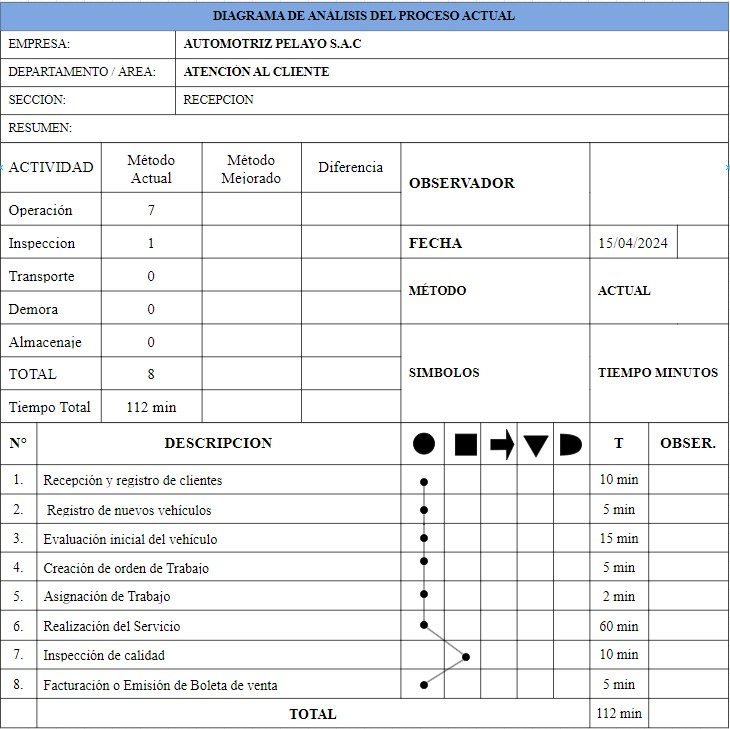
\includegraphics[width=1\textwidth]{imagenes/cap3/DAPcap3captura.jpg}
    %\includegraphics[width=1\textwidth]{imagenes/cap3/DiagramaDOP.png}
    \label{fig:DiagramaDAP}
\end{figure}

\subsection{3.2 Análisis de las causas raíz que generan el problema}
En esta sección del análisis de la situación actual, se procederá a examinar las causas raíz de los problemas detectados en la empresa. Para llevar a cabo este análisis, se utilizará uno de los métodos más reconocidos y utilizados a nivel global en planes de mejora: el método de Ishikawa, también conocido como diagrama de causa-efecto o diagrama de espina de pescado.
\subsubsection*{3.2.1 Método de Ishikawa}
%El Diagrama de Ishikawa es una herramienta visual utilizada para identificar y analizar las posibles causas de un problema específico. En el contexto de este análisis, se aplicará el diagrama de Ishikawa para explorar las diferentes categorías de problemas que afectan el desempeño de la empresa. Cada categoría en el diagrama representa un área potencial de problemas que pueden estar contribuyendo al problema principal, y dentro de cada categoría se identifican las causas específicas.
En el contexto del taller automotriz, se empleará el diagrama de Ishikawa para explorar las diferentes categorías de problemas y sus posibles causas. Cada categoría representa un área potencial de problemas que pueden afectar el desempeño de la empresa. Las escamas principales del diagrama representan estas categorías, mientras que las espinas ramificadas representan las posibles causas dentro de cada categoría.

\begin{enumerate}
    \item Procesos y Procedimientos
    \subsection{Causas:}
    \begin{itemize}
        \item Exceso de tareas en cola: Esto sugiere que hay una acumulación significativa de trabajos pendientes que los operarios deben gestionar, lo cual puede llevar a retrasos y sobrecarga de trabajo.
        \item Gestión de los tiempos de entrega: La ineficaz gestión de los tiempos para completar los trabajos puede resultar en retrasos en la entrega de los vehículos reparados a los clientes.
        \item Retrasos en la facturación: La facturación tardía puede causar problemas de flujo de caja y frustraciones tanto para los clientes como para la empresa.
    \end{itemize}


    \item Infraestructura y Equipamiento
    \subsection{Causas:}
    \begin{itemize}
        \item Infraestructura y equipamiento del taller: Problemas relacionados con la infraestructura física y el equipamiento del taller que podrían afectar la eficiencia y capacidad para manejar la carga de trabajo. Esto puede incluir herramientas obsoletas o en mal estado y una disposición ineficiente del espacio de trabajo.
    \end{itemize}

    \item Recursos Humanos
    \subsection{Causas:}
    \begin{itemize}
        \item Falta de personal capacitado: La carencia de personal con las habilidades y conocimientos necesarios para realizar tareas específicas puede llevar a una disminución en la calidad del servicio y aumentar el tiempo necesario para completar las reparaciones.
        \item Retrasos en la entrega de servicios: La falta de personal adecuado también puede resultar en retrasos en la entrega de los servicios a los clientes.
    \end{itemize}


    \item Materiales y Suministros
    \subsection{Causas:}
    \begin{itemize}
        \item Disponibilidad de piezas y componentes: La falta de disponibilidad de piezas y componentes necesarios para las reparaciones puede resultar en tiempos de espera prolongados para los clientes y afectación en la eficiencia operativa del taller.
    \end{itemize}

    \item Comunicación
    \subsection{Causas:}
    \begin{itemize}
        \item Comunicación con el Cliente: Problemas en la comunicación con los clientes pueden llevar a malentendidos y a una insatisfacción general con el servicio, afectando negativamente la percepción de la empresa.
    \end{itemize}

    \item Gestión de Datos
    \subsection{Causas:}
    \begin{itemize}
        \item Deficiente sistema centralizado de registro: La falta de un sistema eficiente para el registro y gestión de datos puede resultar en duplicidades, errores y dificultades para acceder a información crítica de manera rápida y precisa.
    \end{itemize}

\end{enumerate}

%explicar mejor el diagrama

\begin{landscape}
    \begin{figure}[h]
        \centering
        \caption[Diagrama de Ishikawa]{Diagrama de Ishikawa}
        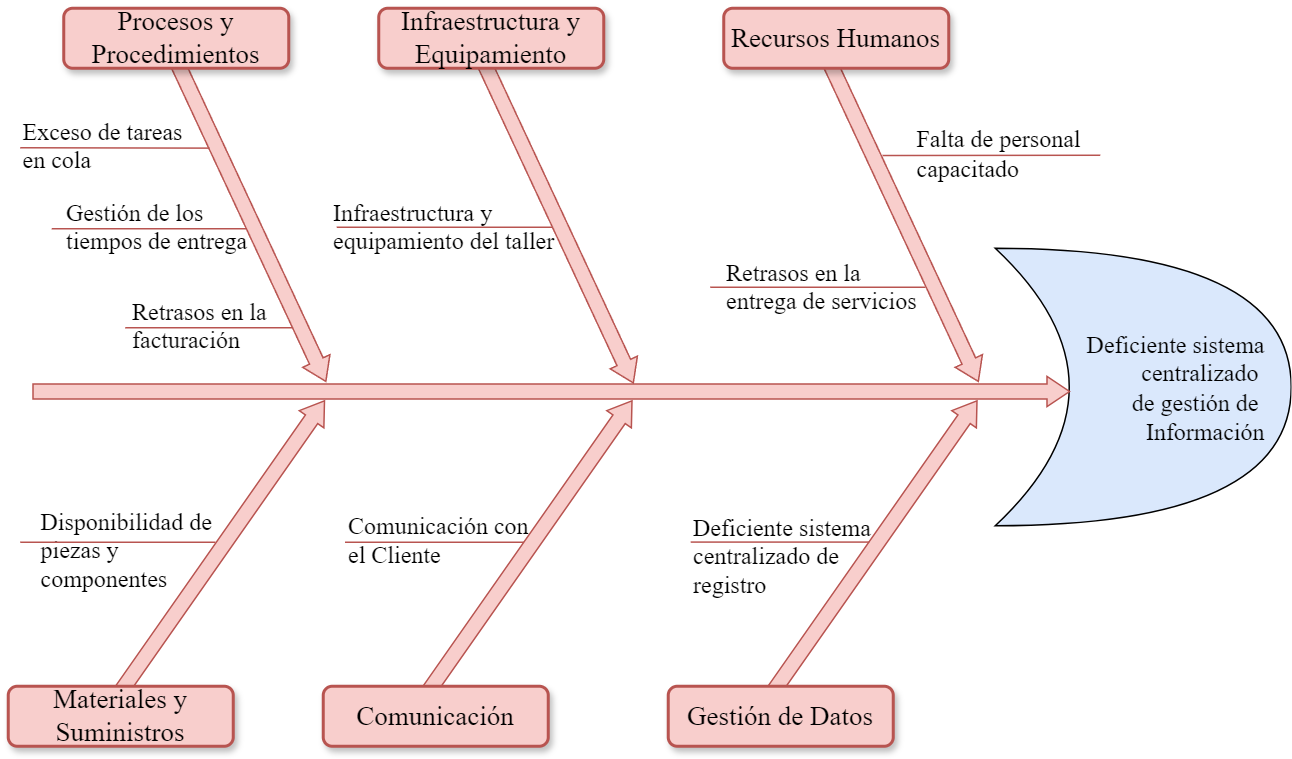
\includegraphics[width=20cm, height=14cm]{imagenes/cap3/IshikawaPescado.drawio.png}
        \label{fig:ishikawa}
    \end{figure}
\end{landscape}

\subsection{3.3 Priorización de causas raíz}
%Se llevó a cabo un análisis detallado de las causas identificadas en el taller, con el objetivo de determinar cuáles tienen el mayor impacto en los problemas observados. Para ello, se utiliza una tabla que muestra la frecuencia de ocurrencia de cada causa raíz y su porcentaje acumulado, lo que permite visualizar de manera clara y concisa cuáles son las principales áreas de mejora.
La priorización de causas raíz es una técnica esencial en la gestión de calidad y resolución de problemas, permitiendo identificar y focalizarse en las causas más significativas que afectan un proceso. En este apartado, se utiliza el Diagrama de Pareto para visualizar y priorizar las causas que generan mayor impacto en el desempeño de un sistema, basándose en el principio de que aproximadamente el 80\% de los problemas son generados por el 20\% de las causas.

\definecolor{ChetwodeBlue}{rgb}{0.556,0.662,0.858}
\begin{table}[H]
\caption[Priorización de causas raíz]{Priorización de causas raíz}
\centering
\begin{tblr}{
  row{1} = {ChetwodeBlue},
  column{1} = {c},
  column{2} = {7.5cm},
  column{3} = {c},
  column{4} = {c},
  column{5} = {c},
  column{6} = {c},
  cell{2}{3} = {c},
  cell{3}{3} = {c},
  cell{4}{3} = {c},
  cell{5}{3} = {c},
  cell{6}{3} = {c},
  cell{7}{3} = {c},
  cell{8}{3} = {c},
  cell{9}{3} = {c},
  cell{10}{3} = {c},
  cell{11}{3} = {c},
  cell{12}{3} = {c},
  hlines,
  vlines,
}
Ítem & Descripcion & Frec & Frec Acum & Porc. & Porc Acum\\
1 & Retrasos
  en la facturación debido al proceso manual y propenso a errores. & 29 & 29 & 25\% & 25\%\\
2 & Deficiente
  sistema centralizado de registro. & 28 & 57 & 24\% & 49\%\\
3 & Dificultades
  para gestionar la demanda en períodos de alta actividad. & 25 & 82 & 21\% & 70\%\\
4 & Exceso
  de tareas en cola para el personal. & 10 & 92 & 9\% & 79\%\\
5 & Deficiencia
  en la gestión de tiempo de los operarios. & 6 & 98 & 5\% & 84\%\\
6 & Deficiencias
  en la infraestructura y equipamiento del taller. & 5 & 103 & 4\% & 88\%\\
7 & Falta
  de personal capacitado para tareas específicas. & 4 & 107 & 3\% & 91\%\\
8 & Retrasos
  en la entrega de servicios. & 5 & 112 & 4\% & 96\%\\
9 & Falta
  de disponibilidad de piezas y componentes necesarios para realizar las
  reparaciones de manera oportuna. & 3 & 115 & 3\% & 98\%\\
10 & Retrasos
  en la entrega de servicios debido a carga de trabajo excesiva & 2 & 117 & 2\% & 100\%\\
 & Total & 117 &  & 100\% & 
\end{tblr}
\end{table}




%La tabla presenta las causas raíz ordenadas según su importancia, destacando aquellas que contribuyen significativamente al total de problemas. Se utiliza el principio de la Ley ABC o Ley 20-80, que sugiere que aproximadamente el 20\% de las causas en estudio generan el 80\% del total de los efectos. En este contexto, se priorizan las causas raíz que representan el 20\% superior en términos de frecuencia de ocurrencia.

%Se elaboro un diagrama de Pareto, para visualizar gráficamente las causas raíz en orden descendente de su frecuencia. Este análisis permite identificar los problemas que requieren mayor atención y desarrollar soluciones inmediatas.

El Diagrama de Pareto presentado, basado en los datos recopilados, permite identificar y priorizar las principales causas raíz de los problemas observados. Este diagrama sigue la regla de Pareto, donde se observa que una pequeña cantidad de causas (aproximadamente el 30\%) contribuye a la mayoría de los efectos (aproximadamente el 70\%).

\begin{figure}[H]
    \caption[Diagrama de Pareto]{Diagrama de Pareto}
    \begin{tabular}{c}
        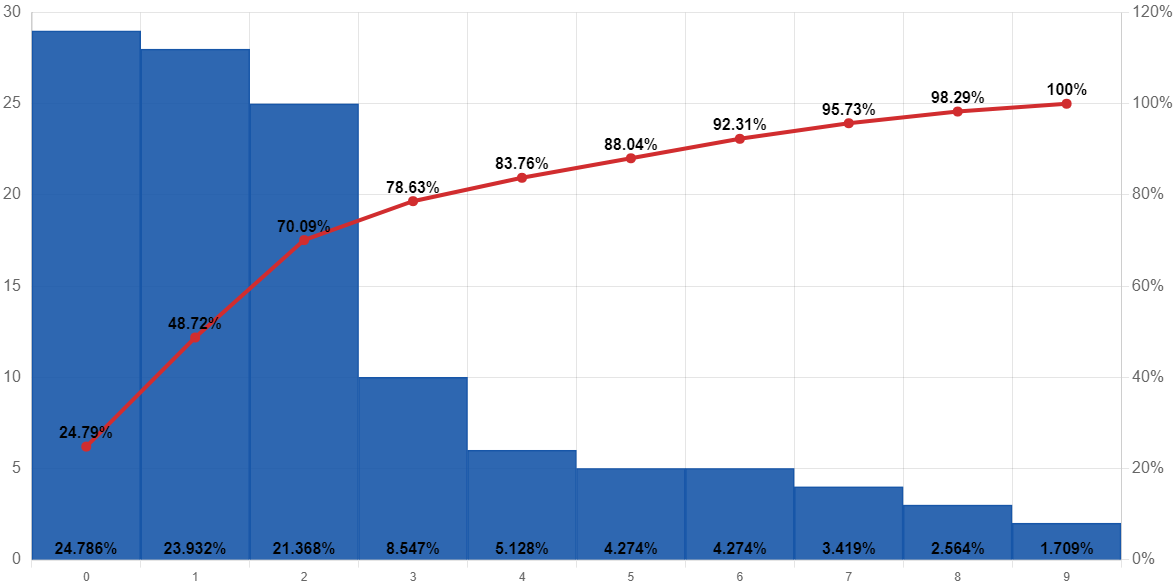
\includegraphics[width=1\textwidth]{imagenes/cap3/diagrama-de-paretoMEj.png}
        %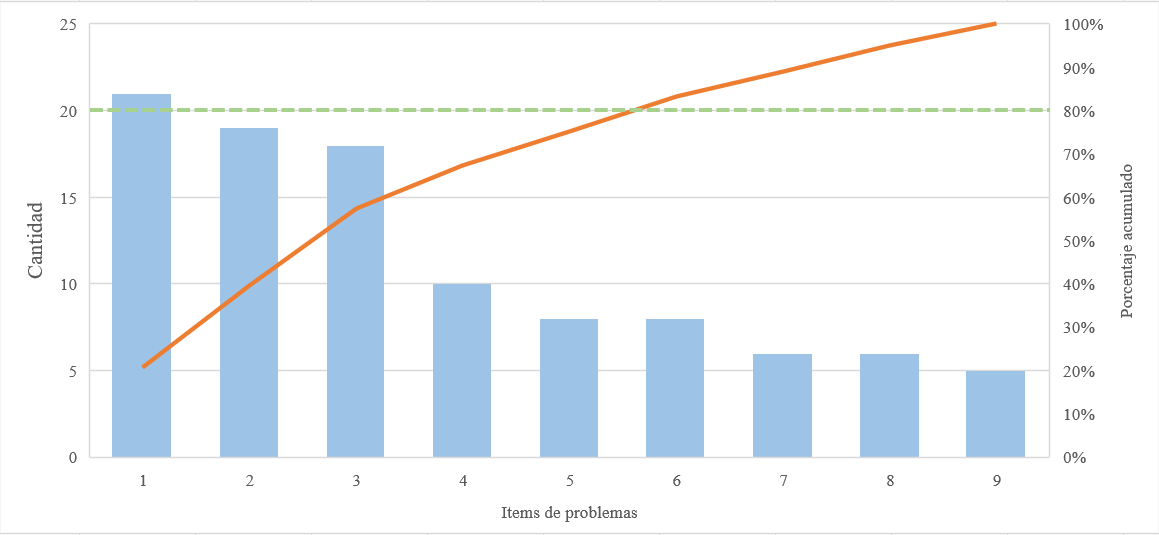
\includegraphics[width=1\textwidth]{imagenes/cap3/Paretov3.png}
    \end{tabular}
    \label{fig:diagramaPareto}
\end{figure}

Como se puede observar en el diagrama, las tres principales causas (retrasos en la facturación, deficiente sistema centralizado de registro y dificultades para gestionar la demanda) contribuyen significativamente a la mayoría de los problemas, acumulando un 70\% de los mismos. Este hallazgo no cumple la regla 80 - 20, pero se acerca y asi se confirma que enfocar los esfuerzos en estas áreas podría resultar en una mejora significativa del sistema general.

%Basado en la información recopilada y los procesos identificados en la empresa antes de la implementación del aplicativo, se observa que existen desafíos significativos en la eficiencia operativa y la gestión de la satisfacción del cliente. Los tiempos de espera prolongados, la falta de coordinación entre los diferentes pasos del servicio y la posible inconsistencia en la calidad del trabajo podrían haber contribuido a una experiencia del cliente insatisfactoria. Además, la falta de una herramienta centralizada para la gestión de los servicios y la comunicación con los clientes podría haber resultado en una falta de seguimiento efectivo y una capacidad limitada para abordar las necesidades específicas de los clientes de manera oportuna. En resumen, el análisis revela áreas clave de mejora que podrían abordarse con la implementación del aplicativo propuesto, con el potencial de optimizar los procesos internos y mejorar la experiencia general del cliente.

%mejorar el diagrama pareto y el diagrama ishikawa.
